\documentclass[tikz,border=2pt]{standalone}
\usepackage{amsmath}
\usetikzlibrary{arrows.meta,decorations.pathreplacing}
\begin{document}
% Grim trigger in the prisoner's dilemma, history with no deviation yet. Conforming: (C,C) forever,
% stage payoffs 3, 3, 3, ... (average 3). One-stage deviation: D only at h^t, then follow s_i, which
% now prescribes D forever: payoffs 5, 1, 1, ... (average (1-delta)5 + delta).
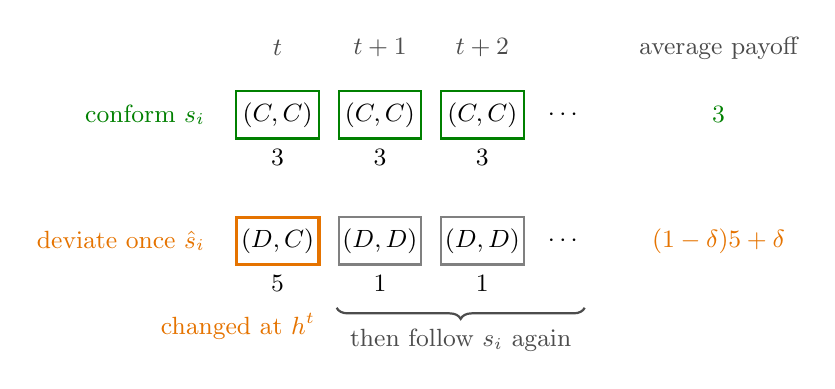
\begin{tikzpicture}[font=\small, >={Latex[length=2mm]},
    cell/.style={draw, thick, minimum width=1.05cm, minimum height=0.6cm, inner sep=1pt}]
  % stage headers
  \foreach \x/\l in {2.6/$t$, 3.9/$t+1$, 5.2/$t+2$}
    \node[gray!60!black] at (\x,0.85) {\l};
  % conforming row
  \node[anchor=east, green!50!black] at (1.8,0) {conform $s_i$};
  \foreach \x in {2.6,3.9,5.2} {
    \node[cell, draw=green!50!black] at (\x,0) {$(C,C)$};
    \node[anchor=north] at (\x,-0.32) {$3$};
  }
  \node at (6.25,0) {$\cdots$};
  % deviating row
  \node[anchor=east, orange!90!black] at (1.8,-1.6) {deviate once $\hat s_i$};
  \node[cell, draw=orange!90!black, very thick] at (2.6,-1.6) {$(D,C)$};
  \node[anchor=north] at (2.6,-1.92) {$5$};
  \foreach \x in {3.9,5.2} {
    \node[cell, draw=gray] at (\x,-1.6) {$(D,D)$};
    \node[anchor=north] at (\x,-1.92) {$1$};
  }
  \node at (6.25,-1.6) {$\cdots$};
  % annotations
  \node[orange!90!black, anchor=north east] at (3.2,-2.4) {changed at $h^t$};
  \draw[decorate, decoration={brace, mirror, amplitude=4pt}, gray!60!black, thick]
    (3.35,-2.45) -- (6.5,-2.45) node[midway, below=4pt] {then follow $s_i$ again};
  % averages
  \node[gray!60!black] at (8.2,0.85) {average payoff};
  \node[green!50!black] at (8.2,0) {$3$};
  \node[orange!90!black] at (8.2,-1.6) {$(1-\delta)5+\delta$};
\end{tikzpicture}
\end{document}
